\section{Literature Review}
\label{sec:bg-litreview}

    \subsection{Mosquito Wingbeat}
    \label{subsec:bg-litreview-mozz}
        
        Early research carried out by \textcite{Landois1866} in 1866 concluded that the flight tone of an insect was due to the number of wing strokes per second, otherwise known as the fundamental frequency or wingbeat of a flying insect. This set the basis for standard practices of determining flight tone by matching a tuning fork to the wingbeat by ear, a method lacking accuracy and objectivity. Only when \textcite{Williams1950} published their work was it understood that the sounds generated during insect flight are 'complex and radically different' from the harmonics produced by a tuning fork. In a study conducted by \textcite{Belton1979} in 1979 on thirteen species of Canadian mosquito, it was found that wingbeat frequencies of each species overlapped but were distinct to at least five other species, and three species were distinct from nine others. However, there was no presence of an overlap between a female and male of the same species. 
        \begin{figure}[ht]
            \centering
            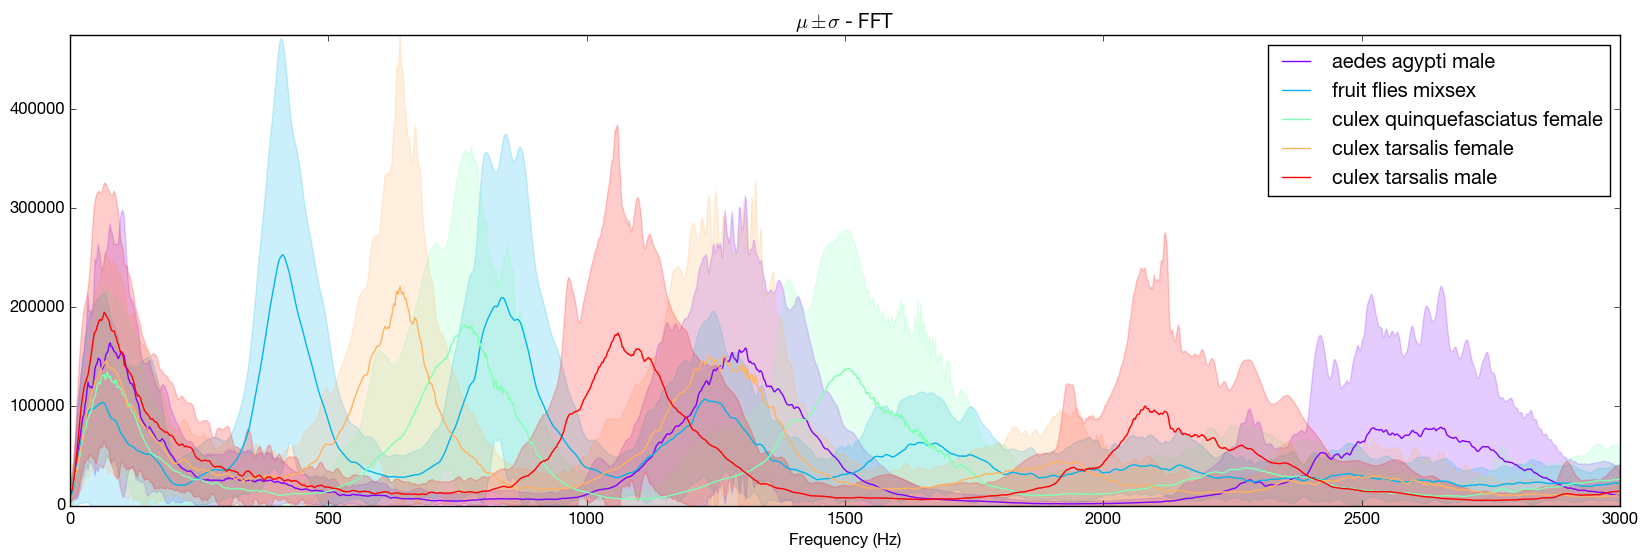
\includegraphics[width=\textwidth]{fft}
            \caption{FFT of four mosquito species, one including both male and female where the sample size is 500 specimens \cite{Chen2014}.}
            \label{fig:bg-litreview-mozz-fft}
        \end{figure}
        Recent research suggests that wingbeat alone, as a scalar, is not adequate to differentiate between mosquito species as there are more than 3,500 species of mosquito with wingbeats mostly in the range of \SI{100}{} -- \SI{1000}{\hertz} \cite{Chen2014}. That range leaves \SI{900}{\hertz} to describe 3,500 species, or \SI{0.26}{\hertz} per species. This is not sufficient considering wingbeats per species can vary as much as \SI{80}{\hertz} either way \cite{Arthur2014}. The use of audio features beyond that of the location of the first harmonic, as well as continuous audio capture of individual species, leads to high volumes of data which substantial information can be extracted from, aiding in this difficult challenge. Figure \ref{fig:bg-litreview-mozz-fft} shows the spectral components of the wingbeat of four species of mosquito, where both male and female specimens have been included for one species. The figure shows clear spectral overlap between classes, making species and gender classification a difficult challenge. The primary focus of this report is to detect mosquitoes over background noise with inexpensive sensors, although species discrimination of the resultant detection pipeline is also be tested using other sets of data.
        %  concern - each sample treated as i.i.d so training over continuous flight of a mosquito will make the classifier broadly detect over lots of frequencies, need to test first     
        % \textcite{Taylor1974} made a surprising discovery in a preceding study that one species (\textit{A. vexans}) would only mate in a cage if another species was present (\textit{A. dorsalis}). \textcite{Belton1979} were able to measure the wingbeat frequencies of both and found that median values were within 5Hz of each other, implying that the sound of the female \textit{dorsalis} may have stimulated the male \textit{vexans} to mate. This research proved that flying insect behaviour, particularly mosquitoes, is governed by sound, among other factors.

    
    \subsection{Current Algorithms and Research}
    \label{subsec:bg-litreview-currentalgs}
        Mosquito detection and identification are active areas of research. The significant majority of research in this field utilises both traditional classification and deep learning techniques on data acquired using opto-acoustic sensors \cite{Batista,Moore1991,Moore1986,Rahuman2016,Moore2002,Li2005,Chen2014,Silva2013}. Higher signal-to-noise ratios (SNRs) are attained using sensors of this type, at the expense of a complex experimental setup requiring mosquitoes to directly intercept optical beams targeted at a phototransistor array, drastically limiting the versatility of the detector as well as limiting recordings to snippets of around \SI{100}{ms}, with no capability to capture continuous flight. Detection of a mosquito in a signal produced by an opto-acoustic sensor is trivial, where an example signal is shown in figure \ref{fig:bg-litreview-currentalgs-opto}.
        \begin{figure}[ht]
            \centering
            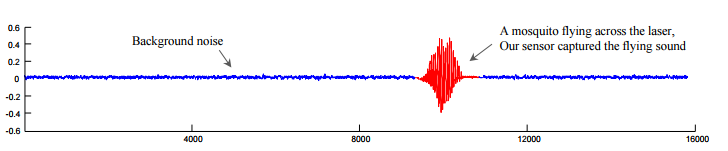
\includegraphics[width=\textwidth]{optoacoustic}
            \caption{Example of an opto-acoustic recording of a mosquito intercepting an optical beam \cite{Chen2014}.}
            \label{fig:bg-litreview-currentalgs-opto}
        \end{figure}
        Mosquito species classification, however, is a complex problem with accuracies around the 80\% region; but these figures are not comparable to the research detailed in this report as the problem of \textit{identification} differs fundamentally from \textit{detection}.
        
        One published study exists that uses purely acoustic data for detection. \textcite{D.R.Raman2007} collect \SI{250}{\hour} of recordings and run an algorithm that looks at spectral energy to determine if harmonic structures are present that align with the characteristic harmonic structure of a mosquito. Although this study shares similarities with the research presented within this report, there are fundamental differences. \textcite{D.R.Raman2007} collect 250 times the volume of data used in this study, which, in addition, is captured in a noise-cancelling environment. Their data is also not labelled, instead the detection algorithm is ran, then the flagged samples are listened to and the false positives are identified. This makes the findings incomparable to this research as the true performance of the detector is unknown.
         % species outside mosquitoes \cite{Chesmore2004,Rahuman2016,Ouyang2015,Moore2002}
        
        The lack of literature on detection in audio signals presents the need for further comprehensive research. Acoustic signals are cheap and easy to obtain; a successful detector on audio alone would have potential for greater global reach than an opto-acoustic-based detector, which requires a more complex setup than a single microphone placed on a surface.